\section{Situationen hos informanterne}
\label{sec:situation}

%indledning
%Vi har valgt at placere dette rige billede, som ses i \figref{fig:rigbillede1}, i starten af dette afsnit fordi vi mener, at den giver et overblik over, hvordan situationen udspiller sig, når man skal forsøge at genbruge madrester.  %LOORT!
I de kommende små afsnit vil vi forklare, hvordan situationen er hos vores to informanter.

\begin{figure}
\centering
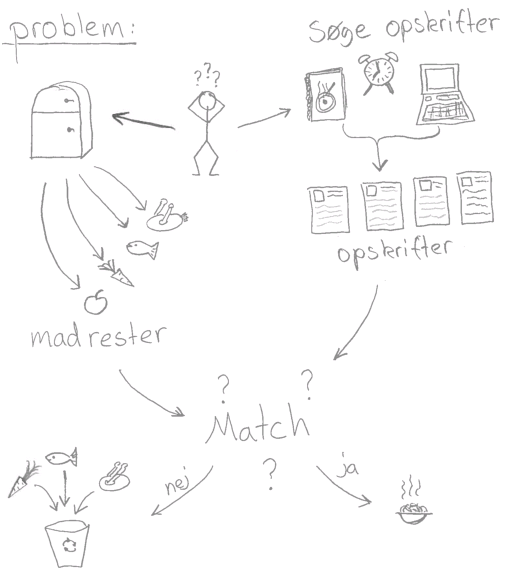
\includegraphics[scale=0.6]{billeder/rigebilleder/problemomraade.png}
\capt{Rigt billede, der visualiserer problemet ved at skulle genbruge madrester.}
\label{fig:rigbillede1}
\end{figure}

Det rige billede i \figref{fig:rigbillede1} viser en person, der ikke har tid eller ressourcer til at finde ud af, hvordan madresterne, som er i køleskabet, kan blive brugt i madlavningen. Dette rige billede er blevet udarbejdet ud fra de initierende samtaler, vi har haft med vores to informanter. Billedet har hjulpet os til at få en forståelse for situationen.

\subsubsection*{Madansvarlige i husstanden}
%situation
Begge informanterne står for madlavningen i deres respektive husstande. De er begge opmærksomme på, at der er dele af aftensmaden, der bliver smidt ud. Denne madspild forekommer selvom, de prøver at genbruge madresterne ved bl.a. at fryse madresterne ned eller genbruge dem den kommende dag i \fx biksemad, supper osv. Det forekommer ofte, at familierne får gårsdagens rester til dagens aftensmad.

\subsubsection*{Madvaner og madlavning}
%madvaner og madlavning
Merete har været vant til at lave aftensmad til to sønner og en datter ud over hende selv og hendes mand. Ægteparrets børn er flyttet hjemmefra, og de spiser derfor sjældent med hos forældrene mere. Det er svært at få mængden af aftensmad til at passe, når der ikke er ligeså mange, som der plejer. Merete er også meget opmærksom på holdbarhedsdatoerne på de forskellige madvarer. Hvis den dato bliver overskredet, så bliver maden smidt ud med det samme.

Derudover forklarer Keld, at han med vilje laver ekstra store portioner til aftensmaden, så familien kan få resterne fra dagens aftensmad den næste dag. Denne strategi benytter Keld sig af, fordi han mener, at der ikke altid er meget tid tilovers til madlavningen. Ægteparret har to små børn, der skal passes og bruges tid på. Udover at tage sig af børnene, så har de også hver deres job, som skal ses til. Derfor er tid ikke noget, som ægteparret har meget af, og de bruger lignende tricks til at bruge mindre tid på madlavningen og mere tid på at være sammen. Det er helt tydeligt, at tiden er en vigtig faktor for Kelds familie, og det er netop derfor, at familien ofte får de samme retter til aftensmad.

\subsubsection*{Indkøb}
%indkøbsliste
Når det kommer til indkøb af madvarer, så er det ikke altid, at der bliver brugt en indkøbsseddel til at planlægge indkøbet. Den person, der har tid, handler ind. Merete og hendes mand kan bedst lide at gå på opdagelse i supermarkedet, og se om de kan finde nogle gode tilbud, som de kan lave noget aftensmad ud af. Keld derimod står altid for indkøb, og han har ofte en plan i hovedet eller en liste i hånden over, hvad han skal have købt med hjem til aftensmaden.

\subsubsection*{Planlægning}
%madplan
Når ugens aftensmad skal planlægges, så benytter hverken Merete eller Keld sig af en madplan. De har ofte idéerne til aftensmaden i hovedet, og madlavningen er rutinepræget. Aftensmaden er meget ensformig, fordi fremgangsmåden er velkendt og derved nem og hurtig at lave. Derudover er det svært for familierne at planlægge tidspunktet for aftensmaden, fordi de alle har jobs, der skal ses til. Derfor ændrer deres planer sig pludseligt, og det vil være svært at styre en madplan, når arbejdstiderne kan variere.
